\documentclass{article}
\usepackage[utf8]{inputenc}

\title{A review on Materials for Drones and Ornithopters}
\author{Aakash Yadav }
\date{March 2019}

\usepackage{natbib}
\usepackage{graphicx}

\begin{document}

\maketitle

\section{Introduction}
In recent years, the use of Unmanned Aerial Vehicles(UAV) is playing important roles in different applications. It is used in many aspects of military and civil broadly, such as aerial photogrammetry, agriculture, warzone, surveillance, traffic and climate monitoring ,and so on. These stealth craft are becoming increasingly popular, not just for war and military purposes, but also for everything from wildlife and atmospheric research to disaster relief and sports photography. Drones are becoming the eyes and ears of scientists by surveying the ground for archaeological sites, signs of illegal hunting and crop damage, and even zipping inside hurricanes to study the wild storms. 
 Unmanned aerial vehicle (UAV) research and development has been growing rapidly over the past decade. 
Commonly known as a drone, a UAV is an aircraft that can perform flight missions autonomously without a human pilot onboard, or can be tele-operated by a pilot from a ground station.
A flapping-wing UAV, also known as ornithopter and usually in about a hand size, is a UAV that generates lifting and forward force by flapping its wings. The aerodynamic modelling and simulation of the ornithopter is much more involved \citep{peterson}.

\begin{figure}[h!]
\centering
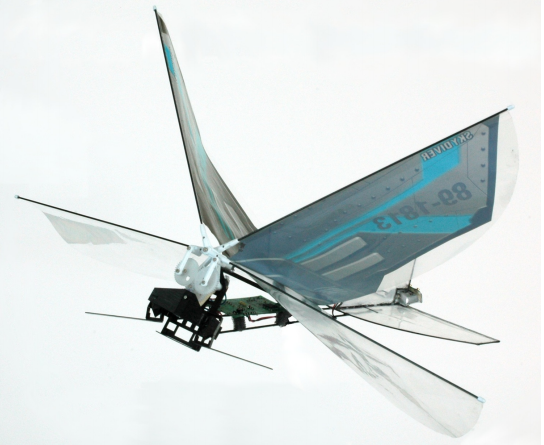
\includegraphics[scale=0.3]{dfm1}
\caption{Ornithopter (courtesy-Peterson et al)}
\label{fig:universe}
\end{figure}

\section{Composite materials }
There is a theory which states that if ever anyone discovers exactly what the Universe is for and why it is here, it will instantly disappear and be replaced by something even more bizarre and inexplicable.
There is another theory which states that this has already happened. 

\section{Design}
There is a theory which states that if ever anyone discovers exactly what the Universe is for and why it is here, it will instantly disappear and be replaced by something even more bizarre and inexplicable.
There is another theory which states that this has already happened.

\section{Conclusion}
``I always thought something was fundamentally wrong with the universe'' 
\citep{Grodzki}
\bibliographystyle{plain}
\bibliography{references}
\end{document}
